\RequirePackage[T1]{fontenc}
\documentclass[nolineno]{ieeeaccess}
\usepackage{cite}
\usepackage{amsmath,amssymb,amsfonts}
\usepackage{graphicx,booktabs,tabularx,array,etoolbox}
\usepackage[hidelinks]{hyperref}
\graphicspath{{figures/}{template/}}
\newcolumntype{Y}{>{\raggedright\arraybackslash}X}
\newcommand{\GG}{GradientGuard}
\newcommand{\WGA}{\operatorname{WGA}}
\newcommand{\SD}{\operatorname{SD}}
\newcommand{\mean}{\operatorname{mean}}
\newcommand{\Dtwenty}{\Delta_{20}}
\setlength{\emergencystretch}{2em}
\widowpenalty=10000
\clubpenalty=10000
\makeatletter
\newlength{\GGabstractwidth}
\setlength{\GGabstractwidth}{\titlewidth}
\addtolength{\GGabstractwidth}{-10pt}
\let\abstractwidth\GGabstractwidth
\def\bodyfont{\rmfamily\fontencoding{T1}\fontseries{m}\fontshape{n}\fontsize{10}{12}\selectfont}
\def\abstractfont{\rmfamily\fontencoding{T1}\fontseries{m}\fontsize{10}{12}\selectfont}
\def\historyfont{\sffamily\fontencoding{T1}\fontseries{m}\fontsize{7}{8.4}\selectfont}
\def\referencefont{\rmfamily\fontencoding{T1}\fontseries{m}\fontshape{n}\fontsize{8.5}{10}\selectfont}
\long\def\@makecaption#1#2{\vskip5pt{\sffamily\fontsize{8}{9.5}\selectfont\noindent\textbf{#1. }#2\par}\vskip4pt}
% Draft metadata replaces the mirror template's example volume/year and DOI.
% The publisher class is retained unchanged; these overrides are manuscript-local.
\def\ps@headings{%
 \def\@oddhead{\hbox to\textwidth{\sffamily\scriptsize Fernando and Edirisooriya\hfill GradientGuard\hfill\mbox{}}}%
 \let\@evenhead\@oddhead
 \def\@oddfoot{\hbox to\textwidth{\sffamily\scriptsize Manuscript v1.1\hfill\thepage}}%
 \let\@evenfoot\@oddfoot}
\let\ps@titlepage\ps@headings
\patchcmd{\@maketitle}{\vss\doifont Digital Object Identifier\space\@doi\vss}{\vss\doifont Exploratory research article\vss}{}{}
\patchcmd{\appendices}{\def\thesectiondis{APPENDIX \Alph{section}}.}{\def\thesectiondis{APPENDIX \Alph{section}}}{}{\errmessage{Appendix compatibility patch failed}}
\makeatother

\begin{document}
\history{Version 1.1, 21 November 2026}
\doi{}
\title{Early Layer Sensitivity for Subgroup Audit Prioritisation with GradientGuard}
\author{\uppercase{Didula Fernando} and \uppercase{Maninda Edirisooriya}}
\corresp{}
\begin{abstract}
Early model measurements may help allocate limited inspection effort to classifiers that later exhibit subgroup failures despite healthy source performance. We investigate layer-wise connection sensitivity as an additional signal for this decision. GradientGuard summarises the distribution of absolute weight--mean-gradient products across shallow and deep network blocks during the first ten percent of training. A staged investigation combines analytical implementation checks, saved-checkpoint probe-partition analysis, a completed outcome experiment with 96 classifiers in 24 configuration families, and post-hoc diagnostics of frozen forecasts. The source-normal held-out cohort contains 36 classifiers and 12 terminal worst-group failures. Six non-slope layer summaries increase average precision from 0.775 to 0.934 and the area under the receiver operating characteristic curve from 0.816 to 0.962 relative to the selected conventional predictor. At twelve inspections, both six- and eight-feature layer variants discover ten failures, compared with eight for conventional and global-sensitivity predictors; this pattern persists across the two probe-panel variants examined. At the original nine-inspection endpoint, all four predictors discover eight failures. Whole-family uncertainty includes zero improvement, and one influential-family omission reverses the larger-capacity comparison. The two added layer-share slopes reach the estimator but add no discovery benefit to the six-feature variant in the primary cohort. These results identify non-slope layer summaries as a promising candidate for independent validation while bounding current claims to an exploratory, benchmark-specific association.
\end{abstract}
\begin{keywords}
Audit prioritisation, connection sensitivity, early training, subgroup robustness, worst-group accuracy.
\end{keywords}
\titlepgskip=-10pt
\maketitle
\pagestyle{headings}

\section{Introduction}
\label{sec:intro}
\PARstart{A}{ggregate} accuracy can conceal large differences between subpopulations. A classifier that performs well on common combinations of object and background may still fail on less common combinations, making source performance alone an incomplete guide to robustness~\cite{sagawa,spare,subpopbench}. When many candidate models are being trained, a developer may have capacity to investigate only a subset in detail. This creates a model-level decision: which apparently healthy runs should receive a later subgroup audit?

We study whether the allocation of early connection sensitivity across network layers provides additional information for that decision. For a frozen model, connection sensitivity is the absolute product of a learned weight and its mean data-loss gradient. Its mathematical primitive is established in pruning and zero-cost model assessment~\cite{snip,zerocost}. A global total records the magnitude of this sensitivity; a normalised layer profile records where it is allocated. These quantities can differ even when model outputs and total weight sensitivity agree. This distinction motivates a predictive experiment, rather than demonstrating that layer profiles encode subgroup reliance.

The research question is: \emph{Can information about which layers a seemingly healthy model depends on help us choose better models to inspect for hidden subgroup failures?} Here, ``depends on'' denotes local loss sensitivity to multiplicative changes in learned weights. It does not imply a causal account of the visual features used by the model. ``Hidden'' refers to unavailable terminal group outcomes at the early decision point; the audit groups are predefined.

This article reports a completed exploratory investigation. A measurement-feasibility study established numerical correctness and useful between-run level variation. A targeted follow-up examined probe partitions, classifier-head aggregation and source-health calibration. A separately authorised outcome proof of concept then trained 96 classifiers to completion. Finally, a bounded post-hoc analysis examined the entire capacity curve and the contribution of slopes without fitting new forecasters. We preserve this chronology: the original outcome experiment designated the eight-feature variant L8 and a 25\% audit capacity as primary, whereas the present interest in L6 and twelve inspections was sharpened after observing those results.

The strongest positive observation is that six layer endpoint, mean and spread features improve held-out ranking metrics and discover two additional failures at twelve inspections. The same layer variants recover all twelve observed failures by seventeen inspections, compared with twenty-five for the conventional predictor. These capacity findings are retrospective and motivate fresh validation. The original nine-audit result remains a tie, and the apparent improvement is sensitive to setting-family composition.

Our contributions are threefold. First, we provide an auditable measurement and experimental pipeline separating implementation correctness, measurement reliability and outcome prediction. Second, we report a family-grouped outcome experiment comparing conventional, global-sensitivity and nested layer representations under a shared early observation budget. Third, we use preserved forecasts to identify which parts of the representation warrant further study: endpoint and prefix-distribution summaries show encouraging exploratory value, while added directional slopes do not improve primary-cohort discovery. The contribution is an empirical investigation of a candidate representation, rather than invention of connection sensitivity or a demonstrated general-purpose shortcut detector.

\begin{figure*}[t]
\centering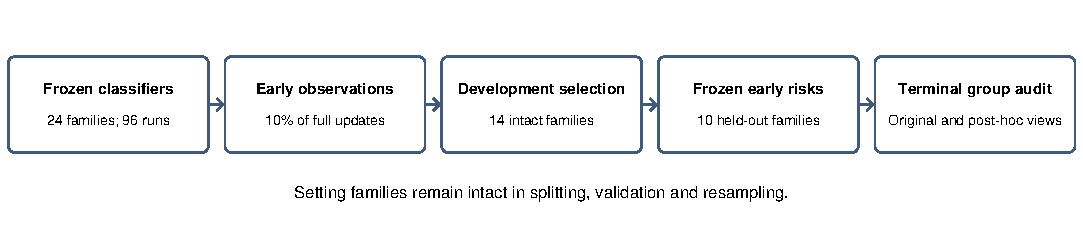
\includegraphics[width=\textwidth]{study_pipeline.pdf}
\caption{Outcome experiment and information boundary. Four related classifiers remain within each setting family. Predictor selection uses development families and validation outcomes; held-out early forecasts precede terminal test evaluation. Later capacity and slope diagnostics reuse the frozen forecasts after outcomes have been inspected.}
\label{fig:pipeline}
\end{figure*}

\section{Related Work and Information Boundaries}
\label{sec:related}
\subsection{Prediction from early training information}
Naik \emph{et al.}~\cite{naik} use early loss, accuracy, gradient signal-to-noise, weight-norm growth, activation saturation and hyperparameters to predict training outcomes. This establishes a substantial conventional-information baseline for any proposed internal feature. Monin~\cite{monin} studies prospective prediction of persistent out-of-distribution degradation from source-side dynamics. The latter's event-conditioned trajectory setting differs from a single fixed early prediction of a completed classifier's subgroup-audit outcome, but changing the target alone does not establish methodological originality.

SPARE~\cite{spare} identifies early output structure associated with spurious correlations and uses importance sampling for mitigation. Our bounded class-conditioned probability-clustering comparator adapts a discovery signal to model-level forecasting; it does not reproduce SPARE's complete algorithm. In particular, this proof of concept uses probability vectors, whereas the relevant published experiments also use logit-based signals. Prediction depth~\cite{depth} is another useful comparator, but is not implemented here. Accordingly, we do not claim improvement beyond prediction depth or beyond a full reproduction of these prior systems.

\subsection{Sensitivity and layer statistics}
SNIP~\cite{snip} supplies the connection-sensitivity primitive. Zero-cost proxies~\cite{zerocost} already aggregate related scores for eventual model-performance ranking. SSNR/T-CET~\cite{ssnr} explicitly studies saliency composition and layer-aware aggregation, while ZiCo~\cite{zico} uses gradient-variation information. Early sensitivity and the observation that aggregation can discard layer information therefore have clear prior art.

Weight-distribution statistics also predict network accuracy~\cite{weights}. Bohadana, Schneider and Katz~\cite{bohadana} investigate performance prediction using weights and gradients; this is especially close technical prior art for internal layer histories. Our literature audit distinguishes the accepted publication record from the accessible associated manuscript version. The present experiment does not implement that full temporal predictor or the richer matched marginal-statistic controls subsequently proposed. Its result is therefore an increment over the implemented conventional/global controls, with sensitivity-specific originality still to be established.

\subsection{Auditing and generalisation measures}
Subgroup discovery and model selection use information regimes different from ours. Domino~\cite{domino} identifies systematic error slices, and SubpopBench~\cite{subpopbench} highlights ordinary worst-class information as a relevant robustness signal. Our early features use ordinary source labels; group annotations are required for historical terminal outcome labels and later evaluation. The system neither discovers arbitrary new groups nor eliminates the need for group-labelled audits.

Studies of generalisation measures~\cite{fantastic,robustmeasures} motivate preserving configuration structure instead of interpreting pooled correlations as universal mechanisms. In our design, the splitting and uncertainty unit is the setting family. Different random seeds within a family, alternative probe panels and overlapping capacity points are not independent experimental settings. These distinctions are central to interpreting the positive signals reported below.


\subsection{The precise gap and candidate contribution}
The distinguishing question is conditional and decision-specific: does a small allocation representation improve the ranking of source-normal completed runs after the information already supplied by ordinary training telemetry and global sensitivity is considered? This differs from proposing another saliency formula. The derivative, normalisation and descriptive summaries are inherited operations; the candidate methodological contribution is their fixed, low-dimensional use in a carefully separated model-audit forecasting task.

Table~\ref{tab:position} makes the comparison boundary explicit. The distinction is an experimentally testable information contract, not a priority claim for all early layer statistics. A method that requires historical audited models is also different from discovering unknown subgroups without such labels. The strongest supported current claim is that this representation merits a matched conditional-addition test, with the existing observations providing a reason to conduct it.

\begin{table*}[t]
\caption{Position relative to close prior work. Distinct prediction targets and information boundaries motivate the experiment; they do not by themselves establish methodological superiority.}
\label{tab:position}
\centering\small
\begin{tabularx}{\textwidth}{>{\raggedright\arraybackslash}p{2.5cm}YYY}
\toprule Prior line & Established information & Distinction investigated here & Evidence needed beyond this pilot\\\midrule
Naik and Monin & Early telemetry and source dynamics predict later outcomes & Fixed 10\%-to-terminal subgroup-audit ranking among source-normal runs & Increment over strong source-side predictors on fresh families\\
SNIP and zero-cost proxies & Weight--gradient saliency and model-ranking totals & Normalised within-model allocation, conditional on total magnitude & A matched global-sensitivity comparison\\
SSNR/T-CET and ZiCo & Layer-aware saliency/gradient aggregation & Six endpoint/mean/spread shares for a completed-run audit decision & Comparison with validated known-aggregation adaptations\\
Weight/gradient predictors & Layer statistics and internal histories predict performance & Coordinate-product allocation as a compact added representation & Rich structural controls with and without exactly the same shares\\
SPARE and subgroup discovery & Early output structure reveals groups for mitigation & Whole-run inspection priority; predefined terminal audit groups & Strong output-signal comparator under matched information access\\\bottomrule
\end{tabularx}
\end{table*}

\section{Connection Sensitivity and Audit Prediction}
\label{sec:method}
\subsection{Frozen-weight measurement}
For labelled source probe $P=\{(x_j,y_j)\}_{j=1}^{n}$ and frozen weights $\theta$, define
\begin{equation}
\begin{aligned}
L_P(\theta)&=\frac1n\sum_{j=1}^{n}\ell(f_\theta(x_j),y_j),\\
g_i&=\frac{\partial L_P}{\partial\theta_i},\qquad a_i=|\theta_i g_i|.
\end{aligned}
\label{eq:sensitivity}
\end{equation}
A gate $m_i$ multiplying one weight gives $\partial L/\partial m_i=\theta_i g_i$ at $m_i=1$. For an entire block, however, a common gate yields the \emph{signed} sum $\sum_i\theta_i g_i$, not the sum of absolute sensitivities. The implementation and finite-difference checks preserve this distinction.

For microbatch $b$ of size $n_b$, the correct probe gradient is
\begin{equation}
g=\sum_b\frac{n_b}{n}\,\nabla_\theta L_b(\theta).
\label{eq:microbatch}
\end{equation}
Absolute products are computed after this signed accumulation. Averaging already-absolute microbatch scores would change the statistic. Our measurement concerns the gradient of mean data loss, not expected per-example saliency; opposing responses may cancel before aggregation.

For included kernel/head weights $W_l$, define
\begin{equation}
\begin{aligned}
S_l&=\sum_{i\in W_l}a_i,\qquad T=\sum_lS_l,\\
q_l&=\frac{S_l}{T+\epsilon},\qquad\epsilon=10^{-12}.
\end{aligned}
\label{eq:shares}
\end{equation}
Biases are excluded from $T$ and measured separately. A record is invalid for nonfinite telemetry, $T=0$, or $\epsilon/(T+\epsilon)\geq0.01$. Probe calls use evaluation mode with gradients enabled, no optimiser update and preserved parameters, training mode and relevant random-number states. Full gradient tensors are discarded after summarisation.

\subsection{Architecture and allocation}
CNN A has three $3\times3$ padded convolutions with widths $3\!\rightarrow\!16\!\rightarrow\!32\!\rightarrow\!64$, trainable biases and rectified linear activations. The first two stages have $2\times2$ max pooling. Global average pooling feeds a biased $64\!\rightarrow\!10$ classifier. There is no batch normalisation or dropout. The shallow block contains conv1 kernels; middle contains conv2 kernels; deep combines conv3 kernels and classifier weights. Individual learned-layer totals and bias diagnostics remain available.

The distinction from norms is algebraically transparent. For one learned layer,
\begin{equation}
S_l=\langle|w_l|,|g_l|\rangle
\leq\|w_l\|_2\|g_l\|_2=U_l.
\label{eq:norm}
\end{equation}
Separate weight/gradient norms do not determine coordinate co-location. For example, $w=(2,1)$ and gradients $(2,1)$ or $(1,2)$ have identical gradient marginals and norms but sensitivity totals five and four. This is an information distinction, not evidence of subgroup prediction. A successful layer predictor could still be explained by generic layer norms, bias behaviour or denominator effects; richer matched controls are needed to resolve that possibility.


\subsection{A falsifiable specificity argument}
For nonzero $U_l$ in \eqref{eq:norm}, write $S_l=U_l c_l$, where
\begin{equation}
c_l=\frac{\langle|w_l|,|g_l|\rangle}{\|w_l\|_2\|g_l\|_2}\in[0,1].
\end{equation}
This elementary factorisation separates ordinary scale from the co-location of absolute coordinate magnitudes. It supplies a reason to measure allocation, but it does not prove that $c_l$ forecasts group failure. Likewise, a normalised profile is compositional: one block's larger share changes the others. The head, biases and shared denominator must therefore be examined before assigning a depth-specific interpretation.

Let $X$ denote the available conventional/global inputs and $Z$ the six L6 share summaries. Predictive improvement of a bounded learner using $(X,Z)$ over one using $X$ supports an increment for that learner and information set. It is not a direct estimate of conditional mutual information or proof that no alternative statistic can recover the same signal. Repeating the addition after expanding $X$ with structural marginals would provide the missing specificity check. This formulation allows a useful layer-information finding even if connection sensitivity ultimately proves replaceable by simpler statistics.

\subsection{Prefix features and nested learners}
At actual full-horizon fractions $t_1,\ldots,t_m$, each signal has endpoint, arithmetic mean, population standard deviation and ordinary least-squares slope
\begin{equation}
\widehat\beta(q)=\frac{\sum_j(t_j-\bar t)(q_j-\bar q)}{\sum_j(t_j-\bar t)^2}.
\label{eq:slope}
\end{equation}
Initialization is diagnostic and excluded from summaries. The 10\% prefix uses six fixed checkpoints; the secondary 5\% prefix uses its available checkpoints. Invalid observations are not interpolated.

The conventional predictor E is selected from compact/rich telemetry with or without output separation and two bounded learner classes. B adds four summaries of total connection sensitivity. L2 adds shallow/deep endpoint shares; L6 adds their four means and population standard deviations; L8 adds their two slopes. Thus L6 contributes exactly six layer-share inputs. Its endpoint is time-anchored; its means and standard deviations do not encode the order of observations. We use ``non-slope'' rather than claiming that L6 contains no history information.

\begin{table}[t]
\caption{Selected source-normal 10\% logistic predictors. Input counts include the shared conventional bank. L8 was the original primary sensitivity learner; L6 was a predefined ablation.}
\label{tab:learners}
\centering\small
\begin{tabular}{lrr>{\raggedright\arraybackslash}p{3.4cm}}
\toprule Predictor & Inputs & $C$ & Added information\\\midrule
E &38&10&Selected compact telemetry\\
B &42&10&Four total-sensitivity summaries\\
L2&44&10&Two block-share endpoints\\
L6&48&0.1&Four block-share means/spreads\\
L8&50&0.1&Two block-share slopes\\\bottomrule
\end{tabular}
\end{table}

\subsection{The audit decision}
For the same eligible candidate pool of $N$ classifiers, rank frozen failure probabilities in descending order, breaking ties by run identifier. Inspect $k=\lfloor0.25N\rfloor$ in the original primary experiment. Let $F$ be the observed number of failures and $D_A(k)$ the failures discovered by predictor A. Report precision $D_A/k$, recall $D_A/F$, random expected discoveries $kF/N$ and oracle ceiling $\min(k,F)$. Precision at $k=0$ is undefined. The comparison is
\begin{equation}
\Dtwenty(A,B)=\frac{20\,[D_A(k)-D_B(k)]}{N}.
\label{eq:gain}
\end{equation}
The original practical target was one extra failure per twenty candidates. Average precision, receiver-operating-characteristic area and Brier score are additional measures, not substitutes for discovery gain.

\section{Experimental Design and Evidence Stages}
\label{sec:experiments}
\subsection{Chronology and scope}
Table~\ref{tab:stages} separates the engineering studies from outcome evidence. The first two stages did not evaluate terminal validation/test outcomes. Following an unresolved health-calibration gate, the 60-epoch outcome study was explicitly authorised as exploratory. It does not retrospectively pass that gate. The final diagnostic stage was planned after held-out outcomes were known and used no new classifier training, forecaster fitting or tuning.

\begin{table*}[t]
\caption{Completed evidence stages and their interpretation. The conditional fresh 18-prefix follow-up was not launched because calibration did not qualify; it is not an executed negative replication.}
\label{tab:stages}
\centering\small
\begin{tabularx}{\textwidth}{>{\raggedright\arraybackslash}p{3.0cm}>{\raggedright\arraybackslash}p{3.3cm}YY}
\toprule Stage & Executed scope & Observation & Evidence boundary\\\midrule
Measurement feasibility & Two conditions; three paired seeds; six early prefixes & Numerical checks pass; selected 256/class deep-slope ratio 3.050141 & Two controlled conditions, not six independent setting families\\
Targeted follow-up & Saved checkpoints; 20 partitions; three calibration trajectories & Original result reproduces; target passes 15/20; no horizon qualifies & Overlapping finite-pool partitions; structural interpretation unresolved\\
Outcome proof of concept & 24 families; 96 complete 60-epoch classifiers & 36 source-normal held-out models, including 12 failures & Family-disjoint evaluation on shared MNIST images\\
Post-hoc diagnostics & Frozen predictions; whole curves; slopes; panels; family influence & Two added discoveries at twelve audits; L6/L8 discovery curves match & Consumed outcomes; hypothesis-generating capacity and representation findings\\\bottomrule
\end{tabularx}
\end{table*}

\subsection{Source construction and reservations}
The outcome study uses official SpuCoMNIST with one class per digit and RGB $28\times28$ inputs~\cite{spuco}. Its 24 setting families are the Cartesian product of alignment probabilities $0.10,0.50,0.80,0.95$, background difficulties MAGNITUDE\_LARGE/MAGNITUDE\_MEDIUM and Adam learning rates $0.0003,0.001,0.003$. Alignment denotes the fraction assigned the class-associated colour; ten-colour independence corresponds to $0.10$, not zero.

The fixed palette, digit identities, ordinary labels and no-noise/no-augmentation choices are verified. Inspection of the pinned generator established that LARGE modifies zero-background pixels over the image, while MEDIUM uses a $4\times4$ corner mask. The official implementation was checked for all 48 seeded source constructions; foreground pixels and labels were preserved. Each construction has 48,004 source-training identities: 256/class are reserved for panel A, another 256/class for B and 128/class for source health, leaving 41,604 training examples. Reservations use ordinary class labels only, with disjoint original MNIST identities and offline background metadata.

Each family has two source constructions and two initialisations per construction. Its four classifiers remain together through splitting, cross-validation and resampling. A configuration-only split with fixed seed 81001 allocates 14 families/56 runs to development and ten families/40 runs to evaluation, with every factor level represented on both sides. These are 24 setting families sharing MNIST, not 96 independent benchmark draws.

\subsection{Training and terminal outcomes}
All models train from scratch with Adam betas $(0.9,0.999)$, no weight decay, batch size 128, no dropped final batch and a constant learning rate. There are 326 updates per epoch, including a final four-example batch. The frozen full horizon is 60 epochs or 19,560 updates. Early observation steps are $196,391,587,978,1467,1956$, corresponding to rounded 1\%, 2\%, 3\%, 5\%, 7.5\% and 10\% fractions. Every non-diverged scientific model completes the full horizon; all 96 did so.

Source-normal eligibility is measured independently at 10\% on the health panel: accuracy at least $0.80$, mean cross-entropy at most $\ln(10)$ and finite required measurements. Ineligible models remain in the full-cohort analysis. The secondary 5\% predictions retain the same 10\%-defined cohort rather than selecting a new favourable population.

Development terminal labels use official validation identities, evaluation labels official test identities. A common outcome panel per difficulty/split uses fixed approximately balanced class/background assignments. Each model has 100 predefined digit/background groups, with observed group sizes 89--135. Define $\WGA=\min_g c_g/n_g$ and failure as $\WGA<0.75$; equality is non-failure. We retain group counts and marginal 95\% Wilson diagnostics. These are not simultaneous uncertainty bounds for the minimum. Fixed 0.70/0.80 sensitivity cutoffs and continuous worst-group regression are secondary. Missing groups, numerical failures and incompleteness are separate statuses, not silently converted to subgroup failures.

\subsection{Telemetry and forecaster selection}
The shared compact bank has learning rate, a fixed activation snapshot and four summaries of nine signals: loss, accuracy, worst-class accuracy, confidence, correct-only confidence, entropy, global mean-gradient norm, weight-norm growth and gradient signal-to-noise. Confidence is maximum softmax probability; entropy uses natural logarithms. Weight growth is $\|w_t\|_2/\|w_0\|_2-1$ over learned weight tensors. The activation snapshot records the nonpositive convolution preactivation fraction, equivalent to zero post-ReLU activations.

The gradient signal-to-noise adaptation uses a fixed layer-stratified subset $\mathcal I$ of up to 4,096 kernel/head coordinates and fixed probe microbatches:
\begin{equation}
\mathrm{GNS}=\frac{1}{|\mathcal I|}\sum_{i\in\mathcal I}\frac{|\bar g_i|}{s_i+10^{-12}},
\label{eq:gns}
\end{equation}
where $\bar g_i$ and $s_i$ are the mean and population deviation of that coordinate's microbatch gradients. This frozen-weight statistic differs from changing-weight epoch telemetry. Rich candidates give loss, accuracy, gradient signal-to-noise and weight growth ten summaries: first, last, change, mean, population deviation, minimum, maximum, area, slope and sign reversals.

The output-separation candidate clusters within-class probability vectors with $k=2$ or $3$, fixed k-means settings, positive silhouette and at least five samples per cluster; otherwise that class has one cluster. It records separation, smallest-cluster fraction and cluster accuracy gap. No group annotations determine these clusters or the observation time.

Regularised logistic regression uses $C\in\{0.1,1,10\}$. Histogram boosting uses depths 1/2/3, 100 iterations, rate 0.05, fixed seeds and disabled early stopping. The historical implementation retained the installed minimum leaf size of 20; this restricts splitting in some small grouped folds and is a comparison limitation. We report it rather than changing defaults after outcomes.

Development selection uses family-grouped out-of-fold discovery at 25\% capacity, average precision as a tie-break and the frozen deterministic candidate ordering. Three stratified grouped folds are preferred, with a two-fold fallback if needed; training and validation folds must contain both outcomes. Imputation, scaling and constant filtering are fit within training folds only. The chosen primary E is compact logistic telemetry without output-separation inputs. All sensitivity variants share this input bank, but their regularisation is selected separately (Table~\ref{tab:learners}). This joint change in input set and fitted regularisation limits direct coefficient-level attribution.

Learning rate is allowed. Alignment, difficulty, generator seeds, subgroup annotations, family/run identifiers, future observations and terminal metrics are excluded from early predictors. A shared diagnostic adds bias-norm/sensitivity endpoints and slopes to E and L8. The selected non-temporal control is logistic B. A final-monitoring reference uses final ordinary health loss/accuracy and learning rate; it receives no terminal subgroup metrics as inputs.

\subsection{Outcome boundary and robustness analysis}
Design and family manifests precede collection. Development classifiers and validation outcomes precede predictor fitting. Saved pipelines, inputs and hyperparameters are frozen before held-out early risks; those risks are frozen before test outcomes are unsealed. The saved audit verifies this order and the hashes. The 21 outcome integration checks and complete-horizon audit support implementation correctness, not predictive superiority.

Panel A is primary. Secondary checks apply frozen A pipelines to panel B and use previously fitted B pipelines with A-selected choices. The post-hoc study loads these existing variants without refitting. It computes every capacity $k=0,\ldots,N$ and marks nine/twelve inspections; twelve is one third for the source-normal pool and 30\% for the full pool.

Uncertainty uses 2,000 paired draws of all ten held-out setting families, seed 130005, keeping nested runs together and recomputing pool size, ranking and fractional capacity. The historical empty/single-outcome exclusion rule is retained for interval comparability: 1,942 draws are valid and 58 invalid. Raw discovery counts remain defined for single-outcome pools. Percentile intervals are conditional on frozen forecasters and observed outcomes, exclude forecaster-selection uncertainty, and are pointwise rather than simultaneous evidence across a searched capacity curve.

Leave-one-family-out analysis removes each of the ten families, including the one with no eligible models. Fractions 1/4 and 1/3 are recomputed using the remaining pool. A family omission is an influence diagnostic, not an independent replication. The post-hoc stage reproduces 27 saved-prediction comparisons to maximum absolute error approximately $1.11\times10^{-16}$ and passes 16 diagnostic checks.

\section{Results}
\label{sec:results}
\subsection{Engineering and measurement feasibility}
The original six-prefix experiment used a 20-epoch planned horizon (6,520 updates) and stopped at 652 updates, approximately two actual epochs. It passed 13 correctness checks and the separately labelled smoke test. The analytical fixture, finite-difference gates, unequal-microbatch accumulation, restricted rescaling, repeatability and monitoring neutrality provide direct checks of the intended statistic. Analytical tolerances are $\mathrm{atol}=10^{-9}$ and $\mathrm{rtol}=10^{-7}$ in float64; float32 accumulation checks use $10^{-6}$ and $10^{-4}$, respectively. No scientific tolerance was relaxed to obtain a pass. Raw slopes from this horizon and the later 60-epoch study are not pooled.

For retained feature $j$ over the six prefixes, sampling noise is $\mathrm{RMS}_r(f_{A,r,j}-f_{B,r,j})/\sqrt{2}$ and spread is the sample standard deviation of $(f_{A,r,j}+f_{B,r,j})/2$. The screen divides spread by the larger of noise and a numerical floor. Floors are $10^{-5}$ for level summaries and $2\times10^{-5}/(t_m-t_1)$ for slopes, raised if repeated-feature noise is larger. Zero-noise, flat and invalid cases are explicitly recorded; these ratios are descriptive engineering screens.

At the selected 256/class budget, the original 10\% deep-slope spread/noise ratio was 3.050141 against a provisional screen of three. Several level features also passed. Ratios compare six-run spread with panel-A/B sampling variation, not population significance. Only three original prefixes met source health. The targeted follow-up reproduced the original feature formulas exactly and remeasured shares to maximum discrepancy approximately $8.33\times10^{-17}$.

Twenty alternative class-stratified partitions recomputed gradients from the saved probe union. The predefined deep-slope target passed in 15/20, short of its prospective 16/20 screen; its ratio median was 3.833 and range 2.086--6.886. These overlapping partitions show sampling sensitivity within one finite pool. Common-denominator conv3, head and combined deep slopes passed 16, 14 and 15 partitions, respectively; convolution-only conv3 passed ten. The uncentred error cross term was positive in all partitions, so net error cancellation did not explain combined reliability. This supports careful aggregation analysis while leaving a layer-specific mechanism unresolved.

The calibration trajectories completed six actual epochs. Neither the two-, four- nor six-epoch observation point passed the unchanged health rule for all three seeds; at four and six epochs two seeds passed. The conditional fresh 18-prefix stage was consequently not launched. The later 60-epoch outcome PoC was explicitly exploratory rather than a validated calibration solution.

\subsection{Outcome support and healthy failures}
All 96 outcome classifiers reached 19,560 updates with finite weights and required telemetry. Table~\ref{tab:support} gives cohort accounting. The source-normal development cohort has eight failures, while the held-out cohort has twelve: healthy source behaviour therefore coexists with the terminal subgroup failures needed to examine the intended decision.

\begin{table}[t]
\caption{Outcome support at the primary 10\% observation. Families can contribute both labels in development; all eligible held-out families have homogeneous binary outcomes.}
\label{tab:support}
\centering\small
\setlength{\tabcolsep}{3pt}
\begin{tabular}{@{}>{\raggedright\arraybackslash}p{2.65cm}rrrr@{}}
\toprule Cohort & Runs & Families & Failures & Non-failures\\\midrule
Development full &56&14&12&44\\
Development source-normal &48&13&8&40\\
Held-out full &40&10&15&25\\
Held-out source-normal &36&9&12&24\\\bottomrule
\end{tabular}
\end{table}

The predefined minimum support convention passes: the held-out source-normal cohort has at least twenty models, six families, five examples per outcome and three families per outcome. Nevertheless, its twelve failures occur in only three eligible families, and none of the nine eligible families contains both outcomes. The result therefore concerns between-setting discrimination under this configuration mixture, with no demonstrated discrimination between successful and failing seeds within a setting. Twelve of all 96 outcomes lie within 0.05 of the failure cutoff, making the retained group-count diagnostics useful for interpretation.

\subsection{Primary capacity and ranking metrics}
At the original nine-audit capacity, E, B, L2, L6 and L8 each find eight of twelve failures (Table~\ref{tab:primary}). Precision is 0.889, recall 0.667 and random expected discoveries three. This is useful prioritisation relative to random selection for the measured pool, shared by the methods; it is not incremental discovery evidence for GradientGuard.

\begin{table*}[t]
\caption{Original primary source-normal held-out results, $N=36$, $F=12$ and $k=9$. L8 is the original primary learner. Layer summaries improve several secondary ranking/probability metrics; the equal discovery counts remain the primary finding.}
\label{tab:primary}
\centering\small
\begin{tabular}{lrrrrrr}
\toprule Predictor & Discoveries & Precision & Recall & AP & AUROC & Brier\\\midrule
E &8&0.8889&0.6667&0.7751&0.8160&0.2036\\
Logistic B &8&0.8889&0.6667&0.7612&0.7847&0.2063\\
Logistic L2 &8&0.8889&0.6667&0.7599&0.7812&0.2061\\
Logistic L6 &8&0.8889&0.6667&0.9336&0.9618&0.1648\\
Logistic L8 &8&0.8889&0.6667&0.9336&0.9618&0.1647\\
Histogram L8 &8&0.8889&0.6667&0.9535&0.9844&0.1531\\
Shared-bias E &8&0.8889&0.6667&0.9182&0.9514&0.1633\\
Shared-bias L8 &8&0.8889&0.6667&0.9304&0.9583&0.1635\\
Final monitoring &4&0.4444&0.3333&0.7203&0.8333&0.1737\\\bottomrule
\end{tabular}
\end{table*}

The secondary ranking improvement is appreciable. L6 increases average precision from 0.7751 to 0.9336 and receiver-operating-characteristic area from 0.8160 to 0.9618 relative to E, with a lower Brier score. L8 has the same reported ranking metrics and a slightly lower Brier score than L6. These observations motivate studying layer endpoint/mean/spread information, while the shared-bias control's strong ranking metrics also motivate richer structural comparisons.

The primary oracle ceiling is nine, leaving E only one additional possible discovery. Its maximum $\Dtwenty$ is therefore $20/36\approx0.556$, below the prospective useful-gain target of one. This limited headroom explains why that target was unattainable in the realised pool at nine audits; it does not convert the observed tie into success.

\subsection{Capacity curves and the twelve-audit signal}
Figure~\ref{fig:curves} presents the full frozen-ranking capacity curves, including the full cohort. In the source-normal pool, L6 and L8 share the discovery curve. Against E they improve at 18 of 37 integer capacities, tie at the other 19 and never lose; against B they improve at 21 and tie at 16. These overlapping points are descriptive, not 18 or 21 independent successful tests. The maximum observed improvement is four discoveries.

\begin{figure*}[t]
\centering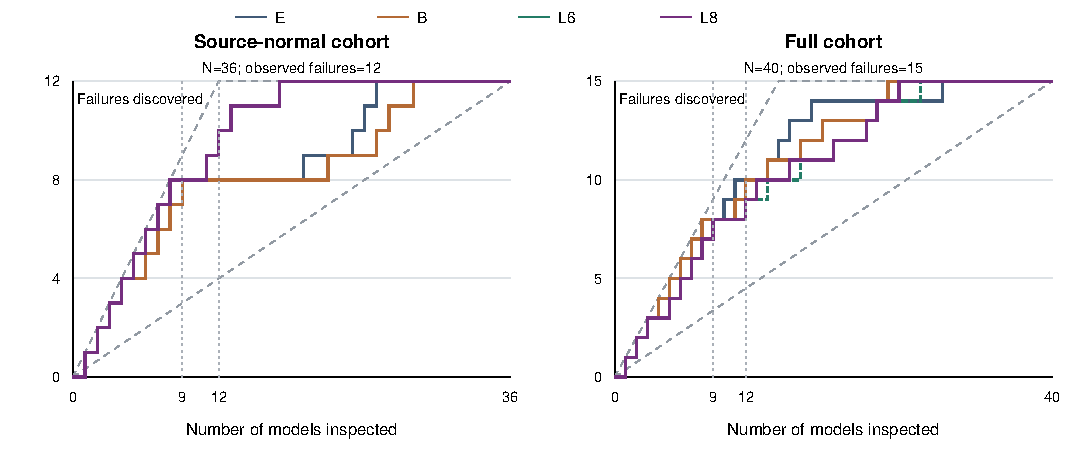
\includegraphics[width=\textwidth]{discovery_curves.pdf}
\caption{Complete discovery curves from frozen primary-panel forecasts. Dashed grey references give random expectation and the oracle ceiling; vertical markers show nine and twelve inspections. In the source-normal pool L6 and L8 overlap. The full-cohort view retains budgets at which conventional prediction performs better. All curves are retrospective descriptive views of already unsealed outcomes.}
\label{fig:curves}
\end{figure*}

At twelve inspections, L6/L8 find ten failures while E/B find eight. Audit precision and failure recall rise from 0.667 to 0.833, and $\Dtwenty=1.111$. The pattern is practically interesting as an observed larger-capacity yield improvement. The paired-family 95\% pointwise interval is approximately $[-1.111,4.444]$, including zero. Twelve inspections were examined post hoc; this result neither replaces the original endpoint nor establishes a reliable gain for a new population.

The retrospective first capacity recovering all twelve failures is seventeen for L6/L8, twenty-five for E and twenty-eight for B. These counts illustrate the shape of the rankings. They are not thresholds available in advance or a validated estimate of deployment audit savings.

\subsection{Probe-panel consistency and family influence}
Table~\ref{tab:panels} shows that the twelve-audit improvement persists with the frozen A predictor on panel B and the existing B refits. At nine audits, the B-refit layer variants find eight compared with seven for E/B, a one-discovery secondary difference. These are encouraging probe-consistency observations using the same classifiers and outcomes.

\begin{table}[t]
\caption{Source-normal discoveries across probe variants. Each paired entry gives E/B versus L6/L8; methods within each pair have the same count. B refits were completed before the diagnostic study.}
\label{tab:panels}
\centering\small
\begin{tabular}{lcc}
\toprule Variant & Nine audits & Twelve audits\\\midrule
A pipeline on A & $8$ versus $8$ & $8$ versus $10$\\
A pipeline on B & $8$ versus $8$ & $8$ versus $10$\\
Existing B refit on B & $7$ versus $8$ & $8$ versus $10$\\\bottomrule
\end{tabular}
\end{table}

Family influence qualifies that consistency. At recomputed one-third capacity, the A predictors produce four positive, five tied and one negative L8--E differences across the ten family omissions (Fig.~\ref{fig:influence}). One positive omission removes the family with no eligible models and leaves the original pool unchanged. Omitting family 12 gives seven discoveries for L8 versus eight for E. The point estimate can therefore depend materially on which settings are present. The existing B-refit variant has eight positive and two tied omissions at this fraction, illustrating panel-specific fitted-model influence rather than independent replication.

\begin{figure}[t]
\centering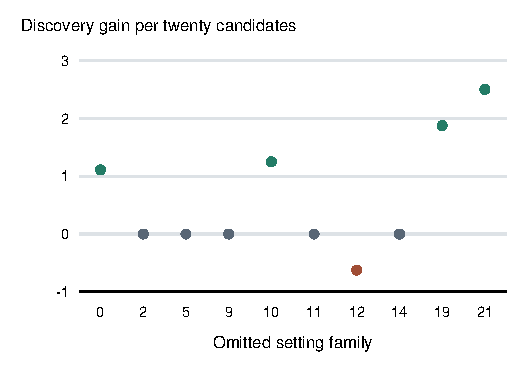
\includegraphics[width=\columnwidth]{family_influence.pdf}
\caption{Leave-one-family-out L8--E gain at $k=\lfloor N/3\rfloor$ after each removal, source-normal A predictions. Capacity and pool size are recomputed. Family 0 contributes no eligible candidate; removing family 12 reverses the comparison.}
\label{fig:influence}
\end{figure}

The full cohort remains a substantive comparison. At its original ten-audit capacity E finds nine failures and L6/L8 eight. At twelve inspections E/B find ten and L6/L8 nine. The source-normal pattern therefore does not extend uniformly to all completed runs; eligibility and configuration composition are part of the observed association.

\subsection{What the slopes contributed}
Both layer-share slopes survive imputation, scaling and constant-feature filtering. They have genuine variation and enter L8. The shallow and deep standardised coefficients are approximately 0.01175 and $-0.00444$, with mean absolute logit contributions 0.00618 and 0.00313. Their small effects in this fitted model cannot be attributed to accidental feature omission.

L6 and L8 probabilities are not identical: the maximum absolute difference is 0.002954, and four rank positions differ. Their label order nevertheless produces the same average precision, receiver-operating-characteristic area and entire primary discovery curve. The selected audit sets are identical at nine inspections; at twelve they overlap in eleven of twelve candidates while retaining the same ten discoveries. Equal ranking metrics do not establish identical complete rankings.

Frozen-input replacement further localises the effect. Replacing one or both slopes by saved development-training reference means sets their standardised components to zero without fitting. The largest probability change is 0.004761 for shallow replacement, 0.002062 for deep replacement and 0.006829 for both. The logit identity holds within about $6.11\times10^{-16}$. No primary-cohort discovery count changes at any budget. This can create unusual feature combinations and is not a causal intervention or a retrained slope-free model. Together with the predefined L6 ablation, it supports prioritising non-slope summaries for a fresh test rather than asserting directional-slope value.

\subsection{Secondary outcomes and structural diagnostics}
The secondary continuous worst-group analysis gives a further modest positive observation (Table~\ref{tab:ridge}). L6 reduces mean absolute error from E's 0.1650 to 0.1588; L8 reaches 0.1473, while its rank correlation is almost unchanged from E. This is a separate regression analysis, with no interval establishing improvement, and does not establish incremental fixed-budget discovery.

\begin{table}[t]
\caption{Secondary source-normal worst-group regression on panel A at 10\%. Lower MAE is better. These ridge models are separate from the binary audit forecasters.}
\label{tab:ridge}
\centering\small
\begin{tabular}{lrr}
\toprule Predictor & MAE & Spearman correlation\\\midrule
E &0.1650&0.7088\\
B &0.1671&0.7006\\
L2&0.1684&0.6810\\
L6&0.1588&0.7036\\
L8&0.1473&0.7090\\\bottomrule
\end{tabular}
\end{table}

Deep-share additivity is verified at every recorded point. At the outcome study's 10\% endpoint on panel A and 256/class budget, none of 96 runs crosses the descriptive head-at-least-50\%-of-deep or bias-at-least-10\%-of-weight-total flags. This narrows two simple endpoint explanations but does not rule out architectural, norm, denominator or bias confounding. Shared bias inputs improve secondary ranking measures without adding primary discoveries. Rich matched weight/gradient-distribution controls remain future work.

At fixed secondary failure cutoffs, E and L8 both discover eight at 0.70 and nine at 0.80 in the primary pool. The limited final-monitoring comparator finds four at nine audits, compared with eight for the early methods. Early observations occur six actual epochs into training, leaving 54 epochs or 17,604 updates of observation lead time. This demonstrates timing and a comparison under the implemented features, not dominance over every final-monitoring strategy or a measured operational benefit.

\section{Computational Cost and Reproducibility}
\label{sec:cost}
The outcome archive records 94.14 minutes of classifier training, 5.20 minutes of six-checkpoint panel-A monitoring, 5.29 additional minutes for panel B, 5.10 seconds of early health assessment and 1.93 minutes of initialization monitoring. Summed classifier invocation wall time is 109.72 minutes. The panel-A path includes ordinary telemetry and clustering as well as sensitivity, so its cost is not an isolated incremental price for GradientGuard. The second panel is research-validation overhead rather than a production requirement.

The largest recorded allocated GPU-memory counter is 567.2 MiB. It is cumulative per process and does not isolate incremental probe memory, other GPU applications or CPU peak memory. Compact source data occupy 57.6 MiB and classifier artifacts 110.3 MiB. Dataset preparation, terminal evaluation and forecaster fitting were not separately instrumented; precise end-to-end component claims would require improved logging.

The numerical stack is Python 3.12.14, PyTorch 2.7.1+cu128, torchvision 0.22.1+cu128 and CUDA runtime 12.8 on an NVIDIA GeForce RTX 5060 Ti. Training uses float32, deterministic operations and no mixed precision or reduced-precision shortcuts. Exact package records, seeds, pinned SpuCo source hashes, configuration snapshots and failed engineering attempts are retained. The later diagnostic environment repair restored a matching interpreter path without changing the 80 dependency records. Reproducibility is conditional on compatible hardware/software, not guaranteed across arbitrary systems~\cite{pytorch}.

The public repository~\cite{repository} contains source, configurations, compact identity manifests, figures, tables, reports, decisions and frozen forecaster artifacts. Environments, raw benchmark downloads, generated numerical dataset arrays and classifier weight/recovery files remain local; a clone therefore requires reconstruction rather than claiming to include every binary. Historical scientific files were imported without line-ending conversion. The manuscript's evidence manifest records the exact archived files used for its tables and figures.

\section{Discussion and Scope of the Findings}
\label{sec:discussion}
The encouraging result is concentrated and interpretable: non-slope layer summaries improve secondary ranking measures and yield more discoveries at several capacities in a source-normal benchmark cohort. Panel-B checks retain the twelve-audit pattern, and the full curve reveals useful ranking structure beyond a single selected point. These observations justify testing the narrower representation with independent configuration families.

The directional interpretation is different. The eight-feature method was the prospective primary candidate, but its two extra slopes contribute no discovery gain over L6 in the primary cohort. Means and spreads are still summaries of a training prefix; the present findings do not establish that endpoint profiles alone suffice, or that all temporal information is unhelpful. The L2--L6 ranking difference motivates a separately controlled endpoint-versus-prefix comparison, while the slope result discourages presenting this pilot as a temporal-direction success.

Sensitivity-specific originality also remains a testable hypothesis. Existing work already uses early telemetry, weights, gradients, saliency totals and layer-aware aggregation. A rich control incorporating ordinary layer norms, parameter/gradient marginals and shared bias diagnostics could explain the observed L6 benefit. A matched control with and without the same six shares would give a stronger conditional-information test. Its results are not part of this article.

The main statistical constraint is family diversity. The held-out source-normal set has only three failure-bearing families and no mixed-outcome family. Shared MNIST and outcome panels add dependence beyond repeated seeds. The bootstrap describes a small frozen-predictor setting mixture, and the influential-family reversal prevents interpreting the two-discovery point estimate as a reliable generalisation improvement. A future design should seek adequate development outcome support and precision before spending its final evaluation budget, without replacing unfavourable families or tuning cutoffs after outcomes.

The practical interpretation is similarly conditional. At the same number of audits the methods spend the same audit capacity; an increased yield is not automatically a monetary saving. Inexpensive benchmark group evaluation may favour auditing every classifier. A realistic use case requires a costly audit or an early reservation deadline, plus monitoring overhead that is justified by the value of additional discoveries. This study demonstrates a ranking decision and observation timing, not operational deployment savings.

The revised proposal describes stronger global and structural controls and a separately designed Waterbirds replication. These remain prospective. No Waterbirds results, pretrained-model transfer evidence, fresh 256-run validation or new forecaster fitting are presented here. The initial nonlinear comparator's small-fold splitting limitation, the bounded probability-based SPARE adaptation and omitted prediction depth further bound claims against strong alternatives. Completing those checks would strengthen the next test, while a result explained by simpler layer statistics would support a narrower contribution.


\subsection{A bounded validation contract for the revised claim}
The existing results select a research hypothesis, not a new primary result on the consumed test set. The next study should designate L6 prospectively and compare three ordered claims: added audit yield beyond conventional telemetry, beyond a strong global-sensitivity predictor, and a conditional increment beyond a rich structural bank. The matched structural pair must use the same development-selected bank, cohort, folds, preprocessing and learner class, adding only $Z$ to the second input set with comparable hyperparameter allowance. Different fitted regularisation is reported as part of the learning procedure, rather than interpreted as an isolated feature intervention.

The structural bank should include layer weight/gradient norms and their products, distribution statistics for parameters and mean-probe gradients, and shared bias diagnostics. These measurements can be validated using existing checkpoints as engineering fixtures; fitting or selecting against their already known held-out labels would remain exploratory. A claimed sensitivity-specific advance requires fresh evaluation of the fixed pair. This comparison directly tests the alternative explanation identified by both reviewers and the literature audit.

Both benchmark protocols, family allocation, eligibility, failure cutoff, audit capacity, estimand and decision rules must precede new evaluation outcomes. The proposed one-third capacity is motivated by consumed diagnostics and must be disclosed as such. The original nine-audit tie remains unchanged. The proposed second-context Waterbirds experiment would use its own development/evaluation separation; it cannot become independent confirmation if its design or predictor choices are changed in response to the new primary test outcomes. Results would remain conditional on two studied benchmark/model contexts, not arbitrary natural-image deployment.

Development checks should assess the number of failure-bearing families, eligibility, mixed-outcome settings, measurement validity, inference calibration and computational cost. Counts of trajectories alone do not establish precision. Readiness must not depend on observing a favourable L6 advantage, and evaluation settings must not be replaced to obtain balance. If support is inadequate or the structural pair shows no credible increment, the contribution is narrowed accordingly. These are prospective requirements; no new control, benchmark result or interval is claimed in this revision.

\subsection{Operational value as an explicit decision test}
An early shortlist is useful when audit slots, specialist time or later data collection must be reserved before terminal outcomes are available. That is an operating scenario to validate, not an assumed property of this inexpensive benchmark. At equal audit count $k$, define a transparent utility scenario
\begin{equation}
\Delta U=v\,[D_{\mathrm{layer}}(k)-D_{\mathrm{base}}(k)]-\Delta C_m,
\end{equation}
where $v$ is an explicitly assumed value per discovered failure and $\Delta C_m$ is incremental monitoring cost. Shared training and equal-count audit costs cancel under this comparison. A positive observed discovery difference supplies a possible benefit region; it does not demonstrate monetary savings without measured cost and a justified value assumption. If exhaustive auditing is cheaper or the baseline reaches the oracle ceiling, the appropriate conclusion is limited operational headroom. This keeps scientific ranking value, early lead time and practical economics separately assessable.

\section{Conclusion}
\GG\ provides a reproducible framework for examining early layer-wise connection sensitivity as a signal for subgroup-audit prioritisation. The completed studies establish engineering correctness of the intended measurement and identify an encouraging non-slope layer-summary pattern in a controlled outcome experiment. In the source-normal held-out pool, L6/L8 improve ranking metrics and find ten failures at twelve inspections compared with eight for conventional/global predictors, with consistent panel checks. The original nine-audit comparison remains a tie, family uncertainty includes zero gain and the added slopes do not improve primary discovery. The next scientific opportunity is a separately frozen evaluation of the six-feature representation against stronger structural alternatives and on a second benchmark context. The present contribution is exploratory evidence and a reproducible test bed for that question.

\appendices
\section{Analytical Fixture and Evidence Access}
\label{app:fixture}
A single positive active channel passes through unit centre kernels and a unit selected head weight; unused connecting weights are zero and unused channels are inactive. Unique pooling maxima and a twice-pooled spatial average of one avoid ambiguity. Bias states $(0,0,0,0)$ and $(0.5,-0.75,0,0.25)$ give selected logit one and the same total weight sensitivity $4|r|$, where $r$ is the selected-logit loss derivative. Their four learned-layer sensitivities divided by $|r|$ are $(1,1,1,1)$ and $(1,1.5,0.75,0.75)$, with ideal three-block shares $(0.25,0.25,0.50)$ and $(0.25,0.375,0.375)$. Epsilon is included in implementation comparisons. This validates possible profile information in CNN A, not a subgroup-accuracy difference or an empirical mechanism.

The evidence directory supplied with the manuscript identifies source hashes and selected tables. The full repository retains all planned original comparisons, full-cohort outcomes and diagnostic curves. The first feasibility, targeted follow-up, outcome PoC and post-hoc attempt identifiers are respectively \texttt{20261116\_01}, \texttt{20261116\_03}, \texttt{20261116\_poc01} and \texttt{20261118\_01}. These identify an audit trail, not four independent confirmations of predictive value.

\section*{Acknowledgment}
OpenAI ChatGPT, accessed through Codex, assisted with drafting and editing the text in Sections I--VIII and the Appendix, and with code used to prepare manuscript tables and vector figures from archived results. AI assistance was also used in developing the archived measurement and experimental software. No additional classifier training or forecaster fitting was performed for this manuscript. The named authors retain responsibility for checking the manuscript, its references and its claims before submission.

\begin{thebibliography}{99}
\raggedright
\bibitem{sagawa} S. Sagawa, P. W. Koh, T. B. Hashimoto, and P. Liang, ``Distributionally robust neural networks for group shifts: On the importance of regularization for worst-case generalization,'' in \emph{Proc. ICLR}, 2020. [Online]. Available: \url{https://arxiv.org/abs/1911.08731}
\bibitem{spare} Y. Yang, E. Gan, G. K. Dziugaite, and B. Mirzasoleiman, ``Identifying spurious biases early in training through the lens of simplicity bias,'' in \emph{Proc. AISTATS}, PMLR, vol. 238, pp. 2953--2961, 2024. [Online]. Available: \url{https://proceedings.mlr.press/v238/yang24c.html}
\bibitem{subpopbench} Y. Yang, H. Zhang, D. Katabi, and M. Ghassemi, ``Change is hard: A closer look at subpopulation shift,'' in \emph{Proc. ICML}, PMLR, vol. 202, pp. 39584--39622, 2023. [Online]. Available: \url{https://proceedings.mlr.press/v202/yang23s.html}
\bibitem{snip} N. Lee, T. Ajanthan, and P. H. S. Torr, ``SNIP: Single-shot network pruning based on connection sensitivity,'' in \emph{Proc. ICLR}, 2019. [Online]. Available: \url{https://arxiv.org/abs/1810.02340}
\bibitem{zerocost} M. S. Abdelfattah, A. Mehrotra, \L{}. Dudziak, and N. D. Lane, ``Zero-cost proxies for lightweight NAS,'' in \emph{Proc. ICLR}, 2021. [Online]. Available: \url{https://arxiv.org/abs/2101.08134}
\bibitem{naik} R. Naik, A. D. Nguyen, and P. K. Singh, ``Predicting deep neural network training outcomes from early training telemetry,'' \emph{arXiv preprint arXiv:2608.03709}, 2026. [Online]. Available: \url{https://arxiv.org/abs/2608.03709}
\bibitem{monin} S. (Alexander) Monin, ``Prospective prediction of OOD degradation from source-side training dynamics,'' \emph{arXiv preprint arXiv:2610.12397}, 2026. [Online]. Available: \url{https://arxiv.org/abs/2610.12397}
\bibitem{depth} R. J. N. Baldock, H. Maennel, and B. Neyshabur, ``Deep learning through the lens of example difficulty,'' in \emph{Advances in Neural Information Processing Systems}, vol. 34, 2021. [Online]. Available: \url{https://proceedings.neurips.cc/paper/2021/hash/5a4b25aaed25c2ee1b74de72dc03c14e-Abstract.html}
\bibitem{ssnr} L. Xiang, R. Hunter, M. Xu, \L{}. Dudziak, and H. Wen, ``Exploiting network compressibility and topology in zero-cost NAS,'' in \emph{Proc. AutoML}, PMLR, vol. 224, pp. 18/1--18/14, 2023. [Online]. Available: \url{https://proceedings.mlr.press/v224/xiang23a.html}
\bibitem{zico} G. Li, Y. Yang, K. Bhardwaj, and R. Marculescu, ``ZiCo: Zero-shot NAS via inverse coefficient of variation on gradients,'' in \emph{Proc. ICLR}, 2023. [Online]. Available: \url{https://arxiv.org/abs/2301.11300}
\bibitem{weights} T. Unterthiner, D. Keysers, S. Gelly, O. Bousquet, and I. Tolstikhin, ``Predicting neural network accuracy from weights,'' \emph{arXiv preprint arXiv:2002.11448}, 2020, revised 2021. [Online]. Available: \url{https://arxiv.org/abs/2002.11448}
\bibitem{bohadana} M. Bohadana, A. Schneider, and G. Katz, ``Neural networks performance prediction using weights and gradients analysis,'' \emph{Transactions on Machine Learning Research}, July 2026. Publication identity verified in the accepted-paper record; accessible associated manuscript: OpenReview 51TWh8tlSy. [Online]. Available: \url{https://www.jmlr.org/tmlr/papers/}
\bibitem{domino} S. Eyuboglu \emph{et al.}, ``Domino: Discovering systematic errors with cross-modal embeddings,'' in \emph{Proc. ICLR}, 2022. [Online]. Available: \url{https://arxiv.org/abs/2203.14960}
\bibitem{fantastic} Y. Jiang, B. Neyshabur, H. Mobahi, D. Krishnan, and S. Bengio, ``Fantastic generalization measures and where to find them,'' in \emph{Proc. ICLR}, 2020. [Online]. Available: \url{https://arxiv.org/abs/1912.02178}
\bibitem{robustmeasures} G. K. Dziugaite \emph{et al.}, ``In search of robust measures of generalization,'' in \emph{Advances in Neural Information Processing Systems}, vol. 33, 2020. [Online]. Available: \url{https://arxiv.org/abs/2010.11924}
\bibitem{spuco} BigML-CS-UCLA, ``SpuCo: Spurious correlation benchmark and toolkit,'' software version 2.0.3, pinned commit \texttt{91842463a577b0a90b4f829fec367308f3052e9f}. [Online]. Available: \url{https://github.com/BigML-CS-UCLA/SpuCo}
\bibitem{pytorch} PyTorch contributors, ``Reproducibility,'' PyTorch 2.7 documentation. [Online]. Available: \url{https://docs.pytorch.org/docs/2.7/notes/randomness.html}. Accessed: Nov. 21, 2026.
\bibitem{repository} D. Fernando, ``GradientGuard research implementation and experiment records,'' GitHub repository, initial archival import commit \texttt{ae2e80c}, Nov. 21, 2026. [Online]. Available: \url{https://github.com/DidulaFernando/GradientGuard}
\end{thebibliography}

\EOD
\end{document}
